\documentclass[12pt]{beamer}
\usepackage{../Estilos/BeamerMAF}
\usepackage{../Estilos/ColoresLatex}

\usefonttheme{serif}
\usetheme{Madrid}
\usecolortheme{whale}
%\useoutertheme{default}
\setbeamercovered{invisible}
% or whatever (possibly just delete it)
\setbeamertemplate{section in toc}[sections numbered]
\setbeamertemplate{subsection in toc}[subsections numbered]
\setbeamertemplate{subsection in toc}{\leavevmode\leftskip=3.2em\rlap{\hskip-2em\inserttocsectionnumber.\inserttocsubsectionnumber}\inserttocsubsection\par}
% \setbeamercolor{section in toc}{fg=blue}
% \setbeamercolor{subsection in toc}{fg=blue}
% \setbeamercolor{frametitle}{fg=blue}
\setbeamertemplate{caption}[numbered]

\setbeamertemplate{footline}
\beamertemplatenavigationsymbolsempty
\setbeamertemplate{headline}{}


\makeatletter
% \setbeamercolor{section in foot}{bg=gray!30, fg=black!90!orange}
% \setbeamercolor{subsection in foot}{bg=blue!30}
% \setbeamercolor{date in foot}{bg=black}
\setbeamertemplate{footline}
{
  \leavevmode%
  \hbox{%
  \begin{beamercolorbox}[wd=.333333\paperwidth,ht=2.25ex,dp=1ex,center]{section in foot}%
    \usebeamerfont{section in foot} \insertsection
  \end{beamercolorbox}%
  \begin{beamercolorbox}[wd=.333333\paperwidth,ht=2.25ex,dp=1ex,center]{subsection in foot}%
    \usebeamerfont{subsection in foot}  \insertsubsection
  \end{beamercolorbox}%
  \begin{beamercolorbox}[wd=.333333\paperwidth,ht=2.25ex,dp=1ex,right]{date in head/foot}%
    \usebeamerfont{date in head/foot} \insertshortdate{} \hspace*{2em}
    \insertframenumber{} / \inserttotalframenumber \hspace*{2ex} 
  \end{beamercolorbox}}%
  \vskip0pt%
}
\makeatother

\makeatletter
\patchcmd{\beamer@sectionintoc}{\vskip1.5em}{\vskip0.8em}{}{}
\makeatother


%Reduce el espacio entre los items de la TOC
\makeatletter
\patchcmd{\beamer@sectionintoc}{\vskip1.5em}{\vskip0.8em}{}{}
\setbeamercolor{section in foot}{bg=ballblue, fg=white}
\setbeamercolor{subsection in foot}{bg=ao, fg=white}
\setbeamercolor{date in foot}{bg=black, fg=white}

\makeatother

\title{Matemáticas Avanzadas de la Física}
\subtitle{Semestre 2023-3 - Intersemestral}

\newcommand\RBox[1]{%
  \tikz\node[draw,rounded corners,align=center,] {#1};%
}

\date{9 de enero de 2023}

\begin{document}
\maketitle

\begin{frame}
\frametitle{Equipo académico}
\begin{center}
\RBox{
M. en C. Gustavo Contreras Mayén \\
\href{mailto:gux7avo@ciencias.unam.mx}{gux7avo@ciencias.unam.mx}
}
\vskip 1cm
\RBox{
M. en C. Abraham Lima Buendía \\
\href{mailto:abraham3081@ciencias.unam.mx}{abraham3081@ciencias.unam.mx}
}
\end{center}
\end{frame}

\section*{Contenido}
\frame{\frametitle{Contenido}\tableofcontents[currentsection, hideallsubsections]}
\fontsize{14}{14}\selectfont
\spanishdecimal{.}

\section{Presentación del curso}
\frame{\frametitle{Contenido}\tableofcontents[currentsection, hideothersubsections]}
\subsection{Objetivos}

\begin{frame}
\frametitle{Objetivos del curso}
En la página de la Facultad, el programa de la asignatura: Matemáticas Avanzadas de la Física se puede consultar 
\href{https://www.fciencias.unam.mx/sites/default/files/temario/610.pdf}{aquí}, y contiene los siguientes objetivos:
\end{frame}
\begin{frame}
\frametitle{Objetivos del curso}
En donde al terminar el curso, el alumno:
\setbeamercolor{item projected}{bg=corn,fg=cordovan}
\setbeamertemplate{enumerate items}{%
\usebeamercolor[bg]{item projected}%
\raisebox{1.5pt}{\colorbox{bg}{\color{fg}\footnotesize\insertenumlabel}}%
}
\begin{enumerate}[<+->]
\item Reconocerá las ideas básicas del análisis de ecuaciones que involucran a funciones de varias variables.
\item Formulará aproximaciones consistentes a soluciones, con el fin de cuantificar los distintos mecanismos de la física que se involucran.
\seti
\end{enumerate}
\end{frame}
\begin{frame}
\frametitle{Objetivos del curso}
\setbeamercolor{item projected}{bg=corn,fg=cordovan}
\setbeamertemplate{enumerate items}{%
\usebeamercolor[bg]{item projected}%
\raisebox{1.5pt}{\colorbox{bg}{\color{fg}\footnotesize\insertenumlabel}}%
}
\begin{enumerate}[<+->]
\conti
\item Consultará la literatura matemática que sea relevante para los problemas de física.
\item Identificará el papel moderno que juegan las funciones especiales, como auxiliares poderosos en el análisis cualitativo de problemas en varias variables.
\end{enumerate}
\end{frame}
\begin{frame}
\frametitle{Objetivo adicional}
También es nuestro objetivo demostrar al alumno que \textocolor{darkmagenta}{las funciones especiales y las transformadas integrales} no son solamente un tema matemático, que involucra las ramas de la geometría diferencial, las ecuaciones diferenciales y el análisis matemático.
\end{frame}
\begin{frame}
\frametitle{Objetivo adicional}
Veremos que \textocolor{darkpastelred}{son las técnicas de estudio fundamentales} en la electrostática, la electrodinámica, la mecánica cuántica en los límites relativista y no relativista, la dinámica de medios deformables, la hidrodinámica clásica entre otras ramas de la física.
\end{frame}
\begin{frame}
\frametitle{Relevancia de la asignatura}
MAF les brindará un manejo más fluido y consistente para lo que van a cursar en el sexto semestre y los tres semestres que les restan para concluir la carrera.
\\
\bigskip
\pause
Es una asignatura con bastante relevancia para la formación del físico.
\end{frame}

\section{Metodología de enseñanza}
\frame[allowframebreaks]{\frametitle{Contenido}\tableofcontents[currentsection, hideothersubsections]}
\subsection{Intersemestral presencial}

\begin{frame}
\frametitle{Situación para el inicio del semestre}
En acuerdo con el programa de horarios el intersemestral 2023-3 tendrá una modalidad presencial.
\end{frame}
\begin{frame}
\frametitle{Días de clase y horario}
Las sesiones se llevarán a cabo los días establecidos: \textbf{lunes, martes, miércoles, jueves y viernes} de 11 am a las 16:30 pm en el aula 301 del edificio nuevo.
\end{frame}

% \begin{frame}
% \frametitle{Plataforma de trabajo}
% Para este curso tanto para las primeras cuatro semanas y en caso de que todo el semestre sea a distancia,  utilizaremos la plataforma Moodle, favoreciendo una estandarización con las demás asignaturas que se imparten en la Facultad de Ciencias.
% \end{frame}
% \begin{frame}
% \frametitle{Plataforma Moodle}
% \begin{figure}
% \centering
% 
\includegraphics[scale=0.2]{Imagenes/Moodle_Ciencias.png}
% \end{figure}
% \end{frame}
% \begin{frame}
% \frametitle{Acceso a Moodle}
% Se proporcionarán las credenciales para ingresar a la plataforma en donde encontrarán las actividades de trabajo, materiales de consulta y referencias adicionales para el curso.
% \end{frame}
% \begin{frame}
% \frametitle{Materiales de trabajo}
% Se contará con materiales que deberán de revisar: en ellos se discute el tema, dentro de los materiales se incluyen ejemplos.
% \\
% \bigskip
% La lectura y trabajo con estos materiales es \emph{obligatoria.}
% \end{frame}
% \begin{frame}
% \frametitle{Materiales adicionales}
% De manera complementaria se dispondrá de materiales adicionales de consulta, en ellos se hará un revisión en particular de un ejercicio o problema.
% \end{frame}
% \begin{frame}
% \frametitle{Materiales adicionales}
% Buscando que el desarrollo se aborde con otro enfoque, pero que complementa lo que hayan revisado en los materiales de trabajo.
% \\
% \bigskip
% Recomendamos mucho que revisen estos materiales adicionales.
% \end{frame}
% \begin{frame}
% \frametitle{Canal de YouTube}
% Se han elaborado videos en donde se trabajan ejercicios y ejemplos para los temas.
% \\
% \bigskip
% \pause
% Dentro de Moodle se estarán incorporando las ligas para el canal de Youtube, de tal manera que podrán revisar los videos en el momento que ustedes consideren oportuno.
% \end{frame}
% \begin{frame}
% \frametitle{Canal en YouTube}
% \begin{figure}[H]
%   \centering
%   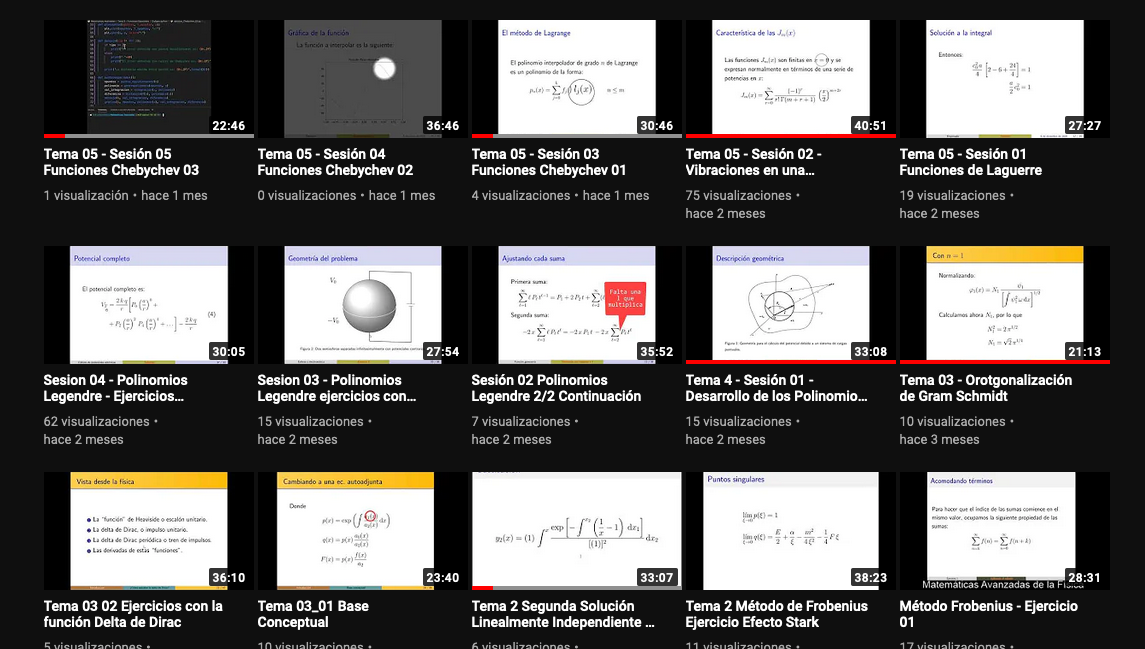
\includegraphics[scale=0.25]{Imagenes/canal_videos.png}
% \end{figure}
% \end{frame}

% \subsection{Tiempo para atender el curso}

% \begin{frame}
% \frametitle{Requerimiento de tiempo}
% De manera independiente a la modalidad de trabajo, deben de considerar \enquote{apartar} tiempo para la asignatura, por lo que hacemos la recomendación de que midan su carga académica durante este semestre.
% \end{frame}
% \begin{frame}
% \frametitle{Comunicación constante}
% Además de contar con los correos electrónicos, se estará utilizando un canal de Telegram para el envío de mensajes generales, así como para notificaciones, avisos, etc.
% \\
% \bigskip
% \begin{figure}
%     \centering
%     
\includegraphics[scale=0.15]{Imagenes/Logo_Telegram.png}
% \end{figure}
% \end{frame}
% \begin{frame}
% \frametitle{Liga y clave para la videoconferencia}
% El envío de la liga y las claves de ingreso a las sesiones de Zoom, se hará por correo, nunca por Telegram.
% \\
% \bigskip
% De esta manera se evita que haya ingresos indebidos a las reuniones.
% \end{frame}
% \begin{frame}
% \frametitle{Material de consulta}
% Se contará con diversos materiales de consulta: artículos, capítulos de libros, etc. que estarán disponibles tanto en la plataforma Moodle como en la nube de Drive, por lo que tendrán oportunidad de consultarlos libremente.
% \end{frame}

\section{Evaluación}
\frame[allowframebreaks]{\frametitle{Contenido}\tableofcontents[currentsection, hideothersubsections]}
\subsection{Esquema de evaluación}

\begin{frame}
\frametitle{Elementos para la calificación}
El porcentaje para cada elemento de evaluación es el siguiente:
\pause
\begin{itemize}[<+->]
\setlength{\itemsep}{0mm}
\item Evaluación semanal: $\mathbf{80\%}$.
\item Ejercicios: $\mathbf{20\%}$.
\end{itemize}
\end{frame}

\subsection{Ejercicios}

\begin{frame}
\frametitle{Ejercicios}
Se presentarán $15$ ejercicios a resolver durante el intersemestral. Los enunciados de lo ejercicios se entregarán durante cada clase.
\\
\bigskip
\pause
Al concluir la semana, se deberá de enviar la solución vía correo electrónico.
\end{frame}
\begin{frame}
\frametitle{Muy importante}
Cada ejercicio aporta un punto, siempre y cuando esté bien resuelto.
\\
\bigskip
\pause
En caso de que que el ejercicio no se haya resuelto debidamente, se otorgará una parte proporcional del punto. Recomendamos ampliamente la solución de todos los ejercicios.
\end{frame}

\subsection{Evaluación semanal}

\begin{frame}
\frametitle{Esquema de evaluación}
Dado el formato del intersemestral, se tendrán tres evaluaciones durante el curso.
\pause
\setbeamercolor{item projected}{bg=darktangerine,fg=darktaupe}
\setbeamertemplate{enumerate items}{%
\usebeamercolor[bg]{item projected}%
\raisebox{1.5pt}{\colorbox{bg}{\color{fg}\footnotesize\insertenumlabel}}%
}
\begin{enumerate}[<+->]
\item Semana 1: Temas 1 y 2.
\item Semana 2: Temas 3 y 4.
\item Semana 3: Temas 5 y 6.
\end{enumerate}
\end{frame}
\begin{frame}
\frametitle{Mecánica de las evaluaciones}
Los enunciados de cada evaluación se entregarán a media semana, de esta manera se tendrá el suficiente tiempo para la solución y entrega del mismo: \pause \textbf{Para las semanas 1 y 2, para el lunes de la siguiente semana}.
\\
\bigskip
\pause
En promedio se incluirán 5 preguntas por cada evaluación.
\end{frame}
\begin{frame}
\frametitle{Ajuste necesario}
En la semana $3$ se tendrá que hacer un ajuste para la entrega de la evaluación por la conclusión del intersemestral.
\end{frame}
\begin{frame}
\frametitle{De cómo se califica}
Durante la calificación de los ejercicios de las evaluaciones y ejercicios \pause \textocolor{ao}{se revisa y se evalúa el proceso de resolución de un problema, es decir, será necesario detallar cada paso en la solución}.
\end{frame}
\begin{frame}
\frametitle{Cómo resolver los ejercicios}
Los ejercicios así como los enunciados de las evaluaciones \textocolor{lava}{tendrán que ser resueltos a mano}, en la solución se deberá de detallar cada paso que se realice.
\\
\bigskip
\pause
No se recibirán soluciones que indiquen comprobaciones hechas en \emph{Mathematica, MatLab, Maple, etc.}
\end{frame}
\begin{frame}
\frametitle{¿Cómo entregar los Ejercicios y Evaluaciones?}
Si cuentan con un escáner, se deberá de digitalizar cada una de las hojas que hayan ocupado en un archivo pdf y enviarlo mediante la plataforma.
\end{frame}
\begin{frame}
\frametitle{¿Cómo entregar los Ejercicios y Evaluaciones?}
En caso de no contar con un escáner para la digitalización de las soluciones, se podrá enviar un archivo con las imágenes de la solución, tomadas con una tableta o el celular.
\end{frame}
\begin{frame}
\frametitle{¿Cómo entregar los Ejercicios y Evaluaciones?}
Se les pedirá encarecidamente, ser lo más claros en la escritura, numeración de las hojas, el orden y limpieza en sus soluciones, para que así recibamos un archivo que nos permita evaluar su trabajo.
\end{frame}

 
% \setbeamercolor{item projected}{bg=columbiablue,fg=cobalt}
% \setbeamertemplate{enumerate items}{%
% \usebeamercolor[bg]{item projected}%
% \raisebox{1.5pt}{\colorbox{bg}{\color{fg}\footnotesize\insertenumlabel}}%
% }
% \begin{enumerate}[<+->]
% \item Transformada de Fourier.
% \item Transformada de Laplace.
% \item Transformada discreta de Fourier.
% \item Transformada rápida de Fourier.
% \end{enumerate}
% \end{frame}

% \section{Cronograma de trabajo}
% \frame{\tableofcontents[currentsection, hideothersubsections]}
% \subsection{Calendarización del curso}

% \begin{frame}
% \frametitle{Calendarización}
% A continuación se presenta el cronograma de trabajo para el curso, durante las 16 semanas del semestre se han distribuido los 6 temas.
% \end{frame}
% {
% \setbeamercolor{background canvas}{bg=}
% \includepdf[pages=1-5]{Calendario_2022_2.pdf}
% }

% \section{Fechas importantes}
% \frame{\tableofcontents[currentsection, hideothersubsections]}
% \subsection{Calendario oficial}

% \begin{frame}
% \frametitle{Fechas importantes}
% %\fontsize{12}{12}\selectfont
% \begin{itemize}[<+->]
% \item \textcolor{red}{Lunes 14 de febrero de 2022. Inicio del semestre 2022-2.}
% \item \textcolor{blue}{Del Lunes 11 al viernes 15 de abril de 2022. Período Vacacional de Semana Santa.}
% \item Martes 10 de mayo de 2022. Día feriado.
% \item \textcolor{red}{Viernes 10 de junio. Termina el semestre 2022-2.}
% \end{itemize}
% \end{frame}
% \begin{frame}
% \frametitle{Fechas importantes - Por confirmar}
% %\fontsize{12}{12}\selectfont
% \begin{itemize}[<+->]
% \item Del lunes 13 al viernes 17 de junio de 2022. \underline{Primera semana de exámenes}.
% \item Del lunes 20 al 24 de junio del 2022. \underline{Segunda semana de exámenes}.
% \end{itemize}
% \end{frame}
\end{document}